\section{Final Prototype}
\label{sec:implementation:prototypes:prototype4}
The purpose of the fourth and final prototype of the iOS application, 
was to connect the concepts from previous prototypes, 
into a final prototype and control actual smart devices.

\subsection{Description}
This iteration of the application removed the need for pressing to start and stop the gesture recognition. 
Instead the user points with the device, 
in order to select one or more smart devices, 
that should be controlled and perform the gesture, 
after a short delay as described in \Cref{sec:detecting-points}.

Furthermore gestures can be configured per action.
An action is something that a smart device can perform. 
Actions for a lamp could be \textit{turn on} or \textit{turn off}.

Each action a smart device can perform can be associated with a gesture. 
Several devices can share a single gesture. 
The screenshots in \Cref{fig:prototype4-app-screenshots} shows how this is configured.

The application shows the following four actions:
\begin{itemize}
\item \texttt{turnOn} for the \emph{Lamp at Dinner Table} device
\item \texttt{turnOff} for the \emph{Lamp at Dinner Table} device
\item \texttt{turnOn} for the \emph{Lamp at Couches} device
\item \texttt{turnOff} for the \emph{Lamp at Couches} device
\end{itemize}

Only the first action, 
\texttt{turnOn} for \emph{Lamp at Dinner Table}, 
has a gesture associated with it. 
The three other actions have no gesture configured, 
and therefore cannot be triggered from the application.
In a realistic scenario, all of the actions would have a gesture associated with them.

Tapping on a one of the action/device combinations presents the gesture picker, 
from which gestures can be added, 
or associated with a device and an action. 
Swiping on a action/device combination, 
lets the user remove an associated gesture.

To test the system on real devices, 
we connected the server to a HomePort server,
which in turn was connected to a small box with two light bulbs and a Phidget interface kit. 
\Cref{sec:serverimplementation} further describes this implementation. 

\subsection{Major Changes}

\begin{itemize}
\item Actual smart devices connected to HomePort are controlled, through the server described in \Cref{sec:serverimplementation}.
\item We removed the need for pressing start and stop, when performing a gesture. Instead the user points with the smarthpone.
\item Gestures can be associated with a device and action.
\end{itemize}

\subsection{Results}

In the fourth prototype all components were connected, 
and the system could be used as a whole. 
Using the fourth prototype we are able to perform tests on the entire system, 
and get a better understanding of how realistic the initial vision of controlling a smart home, 
by pointing at one ore more devices and perform a gesture, is. 
We are also able to get a better overview, 
of which components of the system need improvements in future work.

When using the system with all components connected, 
we found it to be inaccurate. 
We investigated this and found that the inaccurate positioning, 
impacts the accuracy of the entire system almost exponentially, 
as described in \Cref{sec:evaluation:system-correctness}.

Based on this we can conclude that the next step, 
could be to look into alternatives for indoor positioning, 
or possibly substitute the knowledge of the user's position, 
with other information about the context the user is in.
Another possible step to be taken, 
is to port the solution to a wearable.

\begin{figure}[!htb]%
    \centering
    \subfloat{
        \frame{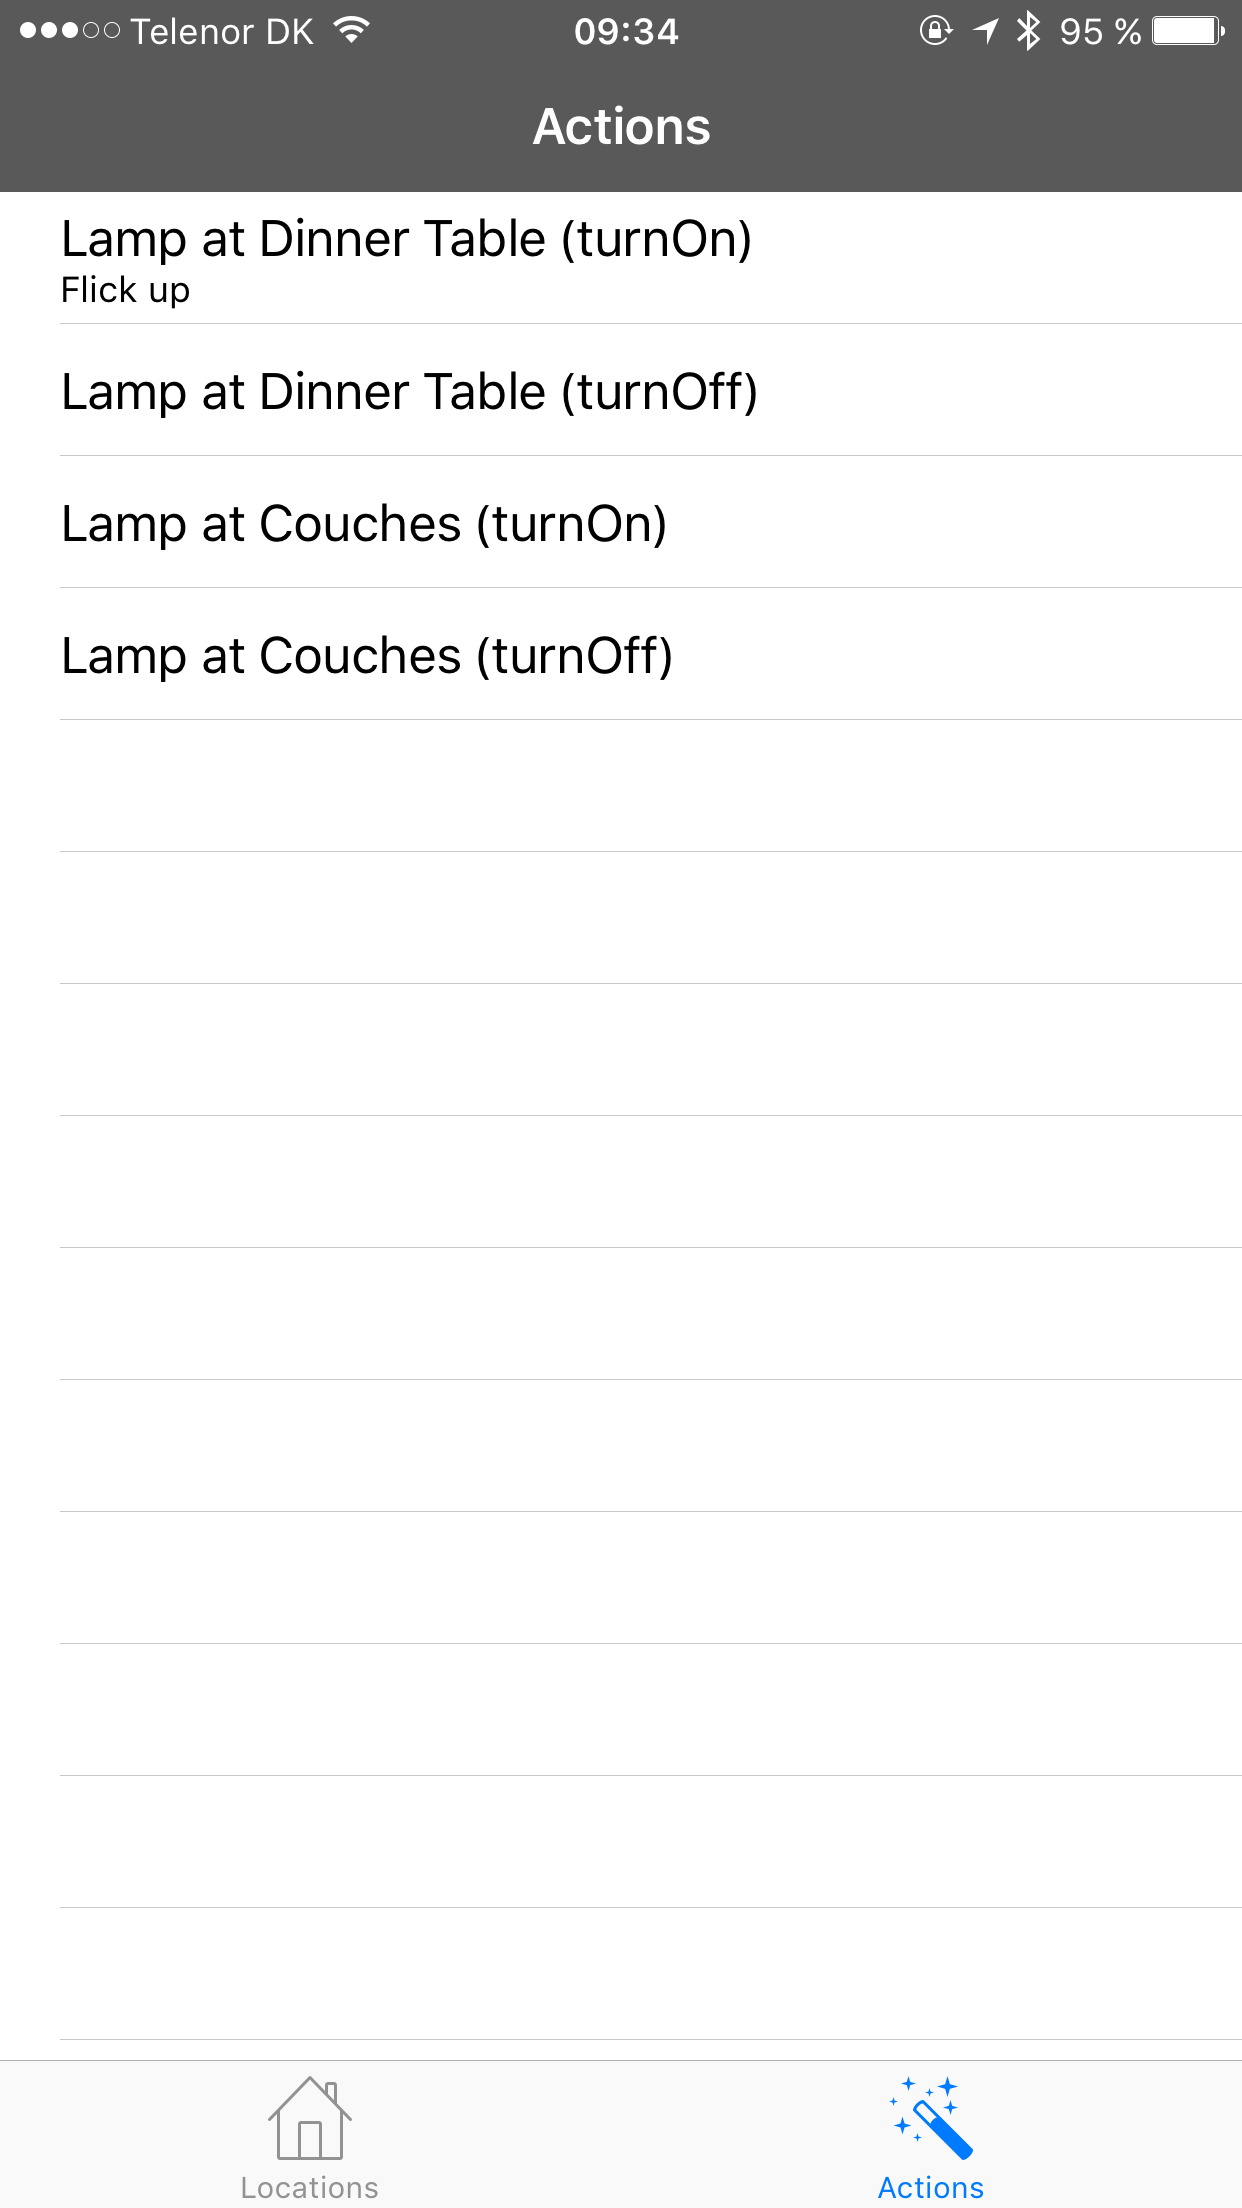
\includegraphics[width=0.3\textwidth]{images/prototype4-1.png}}
    }
    \subfloat{
        \frame{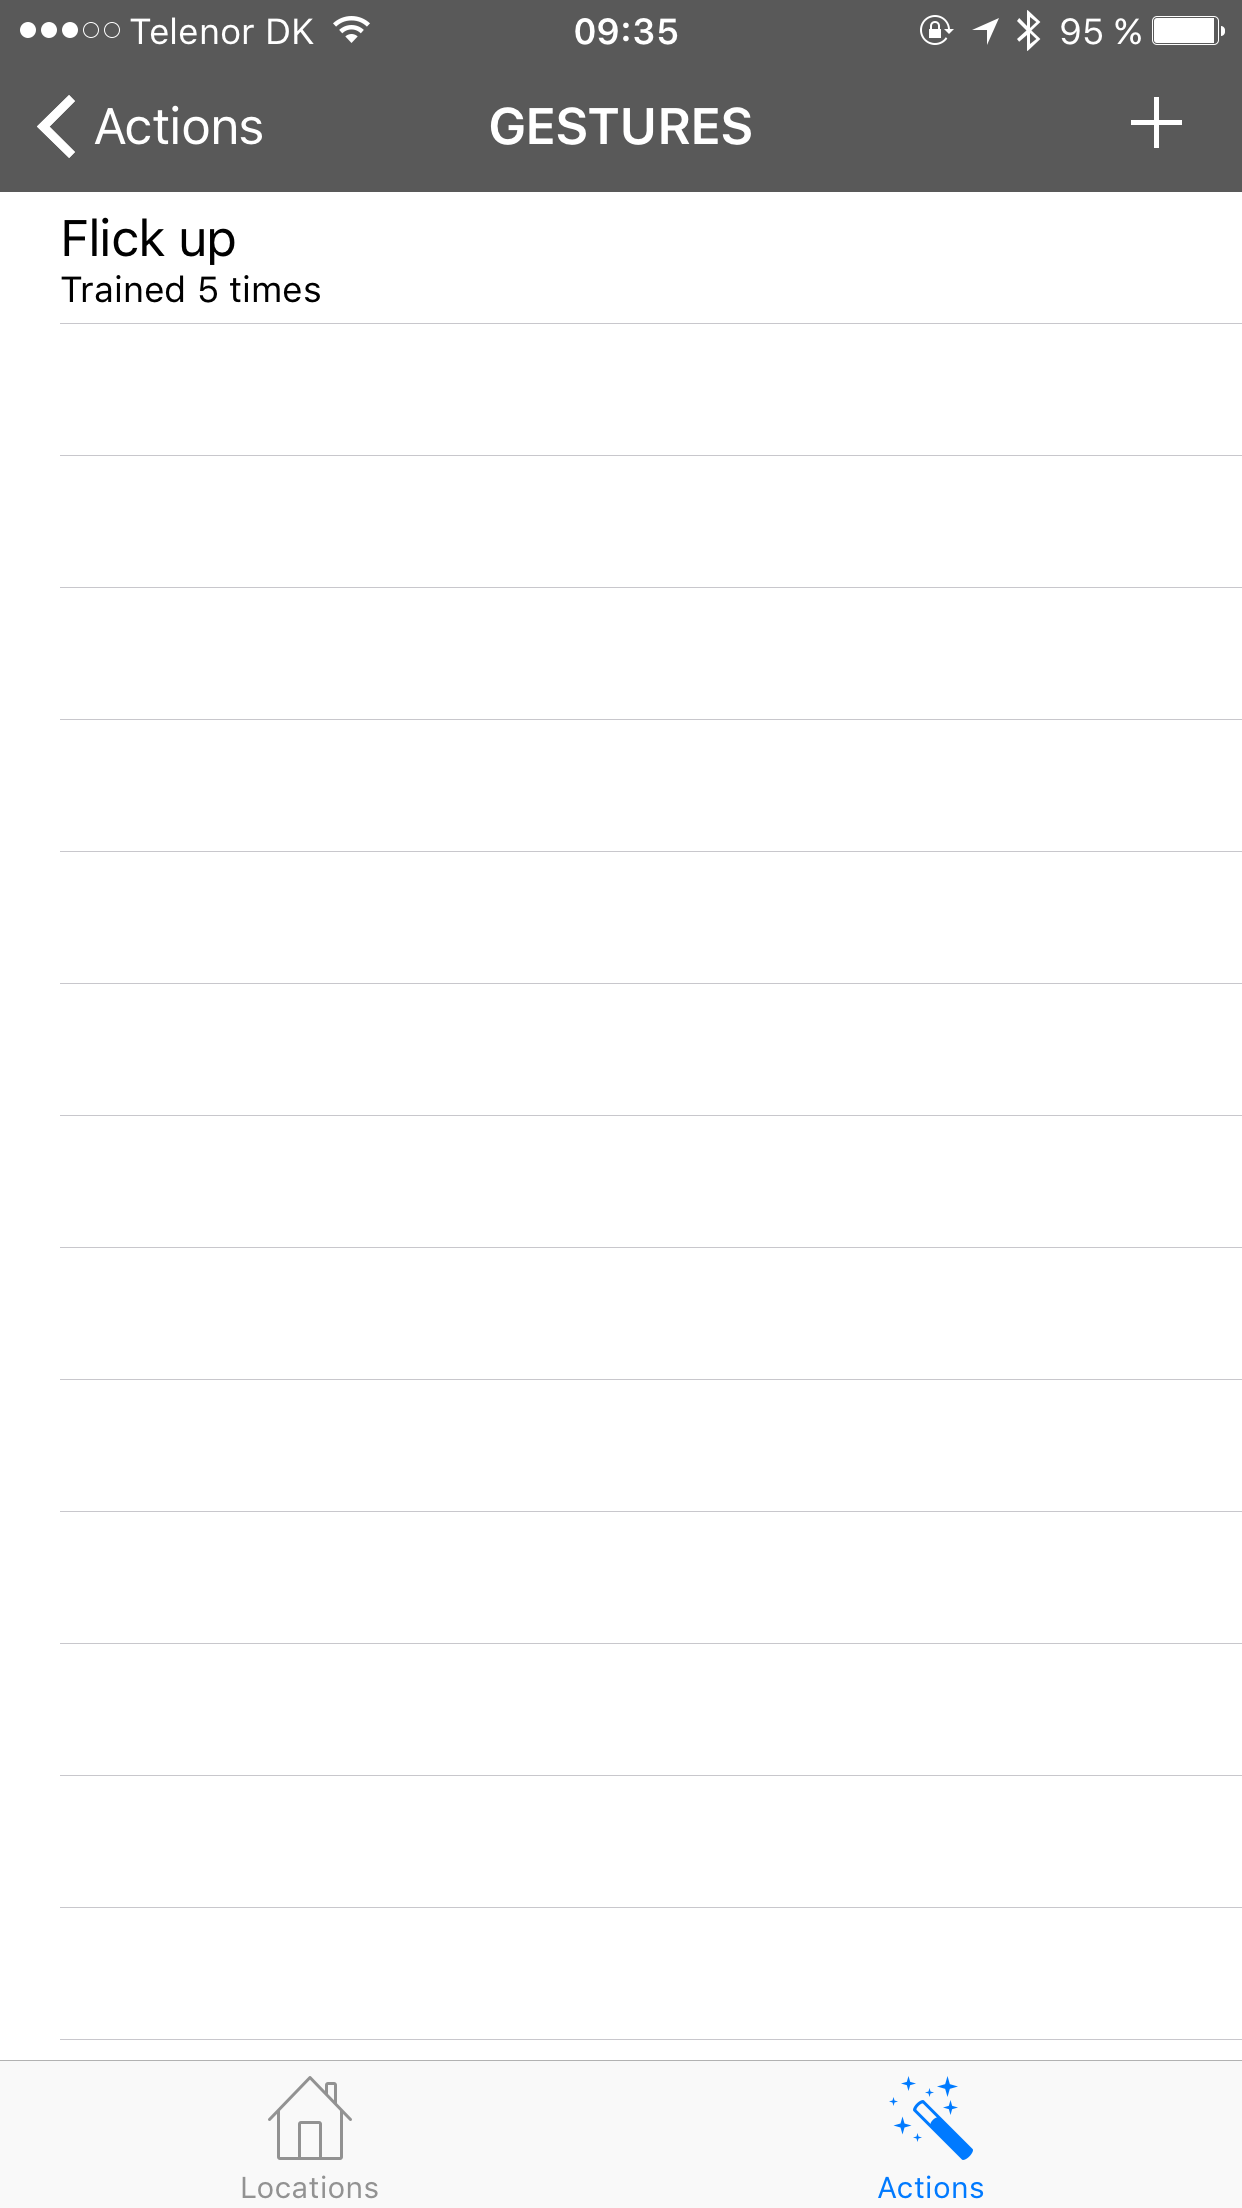
\includegraphics[width=0.3\textwidth]{images/prototype4-2.png}}
    }
    \caption{Screenshots of the fourth and final prototype.}
    \label{fig:prototype4-app-screenshots}
\end{figure}

%%% Local Variables:
%%% mode: latex
%%% TeX-master: "../../master"
%%% End:
